\section{Problemstilling}
Reinseanlegget på Sande blei etablert i 2003. Reinseanlegget er teknisk utdatert og trenger modernisering. 
Styringssystemet er over tjue år gammalt og består av komponentar som ikkje lengre er mogleg å få tak i reservedelar til. 
Mangelen på reservedelar til kritiske komponentar kan gjere at anlegget verte satt ut av drift over lengre tid om noko skjer. 
Bedrifta som leverte styringsanlegget er ikkje lengre i drift, og kompetansen i bedrifta er vekke. 
Dokumentasjonen til anlegget om verkemåte og utforming er mangelfull, og sida bedrifta som leverte anlegget ikkje lengre eksistera er det vanskeleg å oppdrive dokumentasjonen.
Styringa av anlegget er programmert i sekvensar, og alle sekvensane går på tid noko som kan gjere at uheldige situasjonar oppstår sida det ikkje er noko feedback til pls……
Sunnfjord kommune har gitt utrykk for å gå for styresystem løysningar som er «opne» og ikkje gøymd bak lisensar og betalingsmurar.


\begin{figure}[htbp]
    \centering
    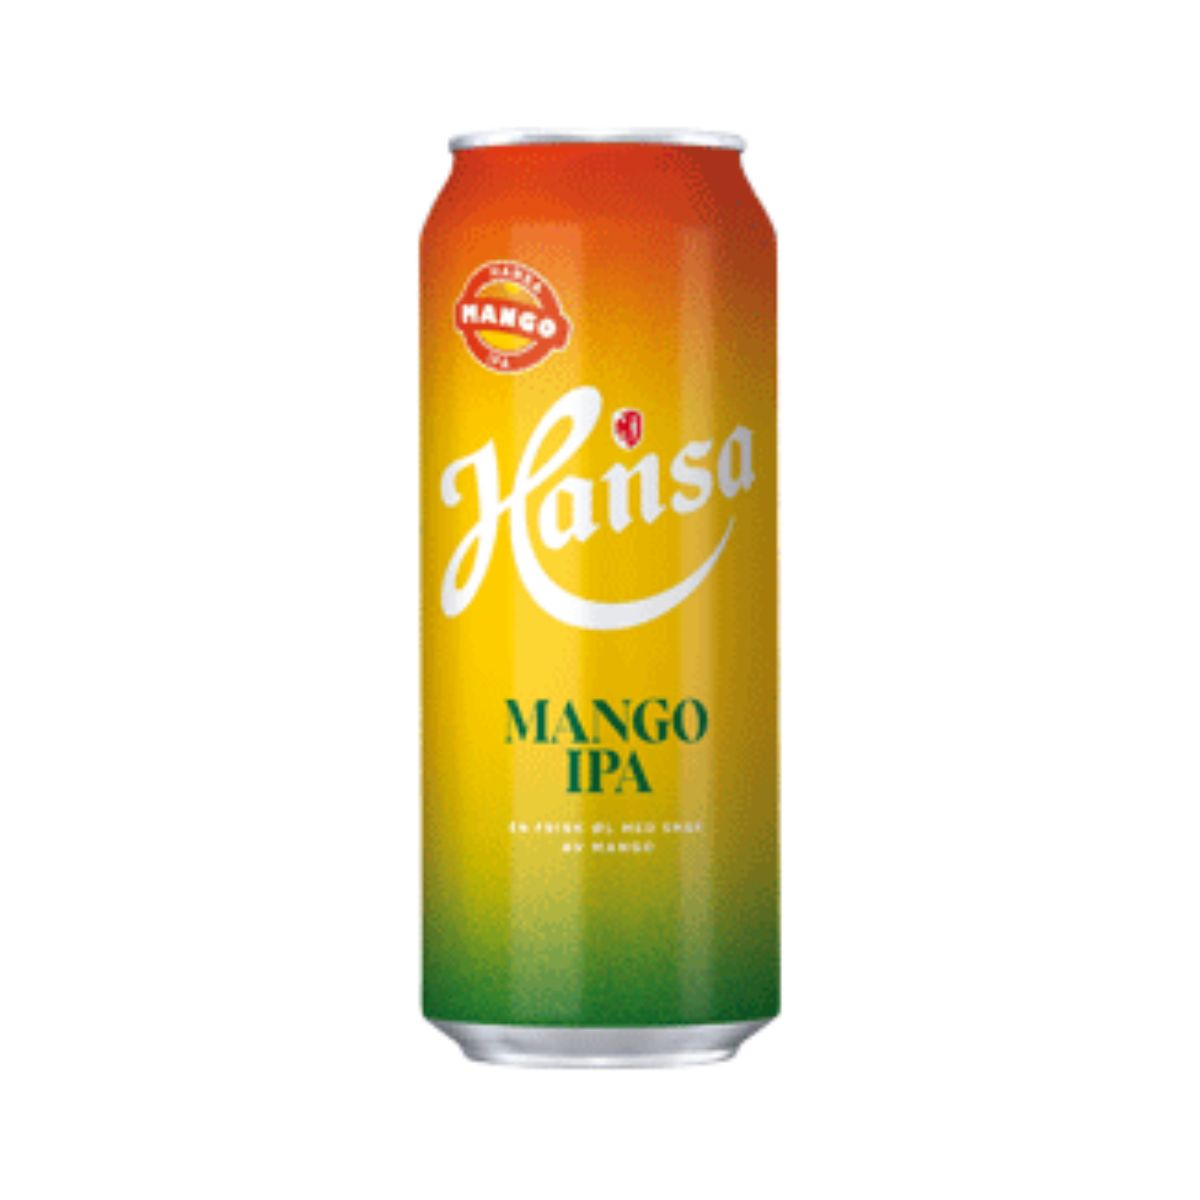
\includegraphics[width=0.5\textwidth]{Bilder/mango.jpg}
    \caption{Mango Ipa We Like}\label{fig:Mango-Loko}
\end{figure}
    